\chapter{Proposed Solutions}

\section{Tools used}
\subsection{3D Slicer}
\textbf{Slicer}, or \textbf{3D Slicer}, is a free, open source software package for visualization and image analysis. It is natively designed to be available on multiple platforms, including Windows, Linux and Mac Os X.

3D Slicer provides image registration, processing of DTI (diffusion tractography), an interface to external devices for image guidance support, and GPU-enabled volume rendering, among other capabilities. 3D Slicer has a modular organization that allows the easy addition of new functionality and provides a number of generic features not available in competing tools.

3D Slicer is built on VTK, a pipeline-based graphical library that is widely used in scientific visualization. In version 4, the core application is implemented in C++, and the API is available through a Python wrapper to facilitate rapid, iterative development and visualization in the included Python console. The user interface is implemented in Qt, and may be extended using either C++ or Python.

Slicer supports several types of modular development. Fully interactive, custom interfaces may be written in C++ or Python. Command-line programs in any language may be wrapped using a light-weight XML specification, from which a graphical interface is automatically generated \cite{slicer}.

For more information on this tool please refer to its official webpage: 

\url{http://www.slicer.org/}

\subsection{ITK}
ITK stands for \textbf{Insight Segmentation and Registration Toolkit}, it's a cross-platform, open-source application development framework widely used for the development of image segmentation and image registration programs.

ITK  is implemented in C++ and it is wrapped for Tcl, Python and Java. This enables developers to create software using a variety of programming languages.

ITK's code is highly efficient, which means that many software problems are discovered at compile-time, rather than at run-time during program execution. It also enables ITK to work on two, three, four or more dimensions.

For more information on this tool please refer to its official webpage: 

\url{http://www.itk.org/}

\subsection{Other Tools}
\subsubsection{Programming Languages}
The programming languages chosen during this project are \textbf{C++} and \textbf{Python}, mainly because they are main languages in which 3D Slicer is written, which means that it was easier to communicate with 3D Slicer by using them.

\subsubsection{MATLAB}
MATLAB is a numerical computing environment and programming language. It allows matrix manipulations, plotting of functions and data, implementation of algorithms, creation of user interfaces, and interfacing with programs written in other languages, including C, C++, Java, and Fortran \cite{matlab}.

MATLAB was used during this project specifically to create and quickly manipulate MRI volume files.

Official website for this tool: \url{http://www.mathworks.com/}

\subsubsection{ParaView}
ParaView is an open-source, multi-platform data analysis and visualization application. ParaView users can quickly build visualizations to analyze their data using qualitative and quantitative techniques.

ParaView was used during this project to visualize the deformation fields produced after the registration of two volumes.

Official website for this tool: \url{http://www.paraview.org/}

\section{Implemented Methods}
During the course of this project two different methods where
implemented, both taking into account previous works about morphometry
and quantification of small changes in volumes.

\subsection{Voxel-based method}
This method was implemented as a \textit{3D Slicer} module with the following steps:
\begin{enumerate}
\item The user selects the base and follow-up volumes to be compared.
\item The user selects the registration method to be used and applies it on the volumes.
\item The module subtracts the base volume and the volume resulting
  from the registration and shows the resulting differences as colored
  layer on top of the base volume.
\end{enumerate}

The registration methods available are: \textit{Affine registration}
(default), \textit{B-Spline deformable registration} and
\textit{BRAINS Demon Warp registration}; all of them available as
already existing modules in \textit{3D Slicer}.

For more information on the registration methods, please refer to
section~\ref{sec:reg_methods}.\\

The subtraction is done pixel-by-pixel and the result produces a label
volume that shows the differences in color over the original base
volume. The chosen color table for the label volume is ``PET-Heat'',
directly available in \textit{3D Slicer}, since it seemed to produce a
volume that was brighter and with easier to spot differences.

\subsubsection{Example}
The following is an example of a volume without mayor differences that
has been modified in order to add some obvious differences in the
shape of circles in both of the original volumes. 

A real user of the application would go through the following steps:

\begin{enumerate}
\item The user selects the \textit{MRIChangeDetectorModule} in \textit{3D Slicer}.

  \begin{figure}[H]
    \centering
    \includegraphics[scale=0.2]{/voxel_example/0.Select.eps}
    \caption{Step 0: Module selection}
    \label{voxel_ex_0}
  \end{figure}
  
\item The user adds the volumes to be analysed.
  
  \begin{figure}[H]
    \centering
    \includegraphics[scale=0.2]{/voxel_example/1.Volumes.eps}
    \caption{Step 1: Adding volumes}
    \label{voxel_ex_1}
  \end{figure}
  
\item The user chooses the registration method to be applied.
  
  \begin{figure}[H]
    \centering
    \includegraphics[scale=0.2]{/voxel_example/2.Registration.eps}
    \caption{Step 2: Registration method}
    \label{voxel_ex_2}
  \end{figure}
  
  
\item The user clicks the button ``Run Quantification'' and the
  program runs the subtraction and creation of label volume.
  
  \begin{figure}[H]
    \centering
    \includegraphics[scale=0.2]{/voxel_example/3.Quantification.eps}
    \caption{Step 3: Running quantification}
    \label{voxel_ex_3}
  \end{figure}
  
\item The program shows the resulting label volume.
  
  \begin{figure}[H]
    \centering
    \includegraphics[scale=0.2]{/voxel_example/4.Result1.eps}
    \caption{Step 4: Quantification result}
    \label{voxel_ex_4}
  \end{figure}

  Note that the resulting differences look like rings. This is the
  expected result because both of the original volumes were modified
  by adding circles of distinct sizes.
  
\item The user can now watch the label volume on top of the original
  volume and move the planes as he wishes.
  
  \begin{figure}[H]
    \centering
    \includegraphics[scale=0.2]{/voxel_example/5.Result2.eps}
    \caption{Step 5: User visualization}
    \label{voxel_ex_5}
  \end{figure}

\end{enumerate}


\subsubsection{Technical Details}
The user interface of the module is written in \textit{Python} using
some libraries from \textit{Qt} and \textit{CTK}, being
\textit{ctkWorkflowWidgetStep} from \textit{CTK} the most important
since it allows the creation of a ``step-by-step'' wizard.\\


The part of the module in charge of the subtraction of volumes is
written in \textit{C++} using \textit{ITK}.

The subtraction is done using the ITK filter
\textit{AbsoluteValueDifferenceImageFilter}, which computes the
difference between each two pixels and then calculates the absolute
value of the result. This allows the module to detect all the possible
differences between the volumes, regardless of the sign of the
resulting values.\\


\subsection{Tensor-based method}
This method was also implemented as a \textit{3D Slicer} module with the following steps:
\begin{enumerate}
\item The user selects the base and follow-up volumes to be compared.
\item The user selects the displacement field smoothing sigma to use during the registration and runs it.
\item The user selects the percentage of growth and shrinkage that he
  would like to see and runs the measurements. The module shows the
  result as a colored layer on top of the base volume.
\end{enumerate}

The registration method that is used in this case is \textit{BRAINS
  Demon Warp Registration}, for more information on this method please
refer to section \ref{sec:demon_warp}.\\

The \textit{displacement field smoothing sigma} is a Gaussian
smoothing value to be applied to the output deformation field at each
iteration of the registration process. Increasing this value produces
deformation fields that are smoother and where the vector values are
less prone to show big changes over very small movements in the field.

The default value for the smoothing sigma is $1.0$; however, according
to our experiments, to produce deformation fields that are smooth
enough the value should be between $2.0$ and $3.0$.\\

The module also allows the user to choose the percentage of the values
of the \textit{Jacobian determinants} that will be shown in the final
result. Since there are two types of values (corresponding to growing
and shrinking of the original volume), there is also two values to
select. For example, if the user chooses to view $50\%$ of the growth
values, only half of the values that represent growth in the
deformation field will actually be shown on the resulting label map.\\
% TODO something about which values are better?

Once the user has seen the results with certain percentages, the
module can be run again with a new set of parameters in order to get
better results.

\subsubsection{Example}
The tensor-based method will be applied to the same volumes used in
the previous example. A real user of the application would go through
the following steps:

\begin{enumerate}
\item The user selects the \textit{TensorMRIChangeDetectorModule} in \textit{3D Slicer}.

  \begin{figure}[H]
    \centering
    \includegraphics[scale=0.2]{/tensor_example/0.Select.eps}
    \caption{Step 0: Module selection}
    \label{tensor_ex_0}
  \end{figure}
  
\item The user adds the volumes to be analysed.
  
  \begin{figure}[H]
    \centering
    \includegraphics[scale=0.2]{/tensor_example/1.Volumes.eps}
    \caption{Step 1: Adding volumes}
    \label{tensor_ex_1}
  \end{figure}
  
\item The user chooses the deformation field smoothing sigma and begins the registration. 
  
  \begin{figure}[H]
    \centering
    \includegraphics[scale=0.2]{/tensor_example/2.Registration.eps}
    \caption{Step 2: DEMONS Warp Registration}
    \label{tensor_ex_2}
  \end{figure}
  
  
\item  The user chooses the percentage of growth and shrinkage to
  use in the output label map and clicks the button ``Run Tensor
  measurements'' to initiate the tensor calculations.

  \begin{figure}[H]
    \centering
    \includegraphics[scale=0.2]{/tensor_example/3.Quantification.eps}
    \caption{Step 3: Running tensor measurements}
    \label{tensor_ex_3}
  \end{figure}
  
  The volume that can be observed in the image is the deformation
  field produced by the registration from the previous step.

\item The program shows the resulting label volume directly on top of the original volume.
  
  \begin{figure}[H]
    \centering
    \includegraphics[scale=0.2]{/tensor_example/4.Result1.eps}
    \caption{Step 4: Quantification result}
    \label{tensor_ex_4}
  \end{figure}
  
\item The user can now move the planes and visualise the volumes as desired.
  
  \begin{figure}[H]
    \centering
    \includegraphics[scale=0.2]{/tensor_example/5.Result2.eps}
    \caption{Step 5: User visualization}
    \label{tensor_ex_5}
  \end{figure}


\item The user can change the percentage numbers depending on what he
  or she wants to see and re-run the module by clicking the button
  once again.
  
  \begin{figure}[H]
    \centering
    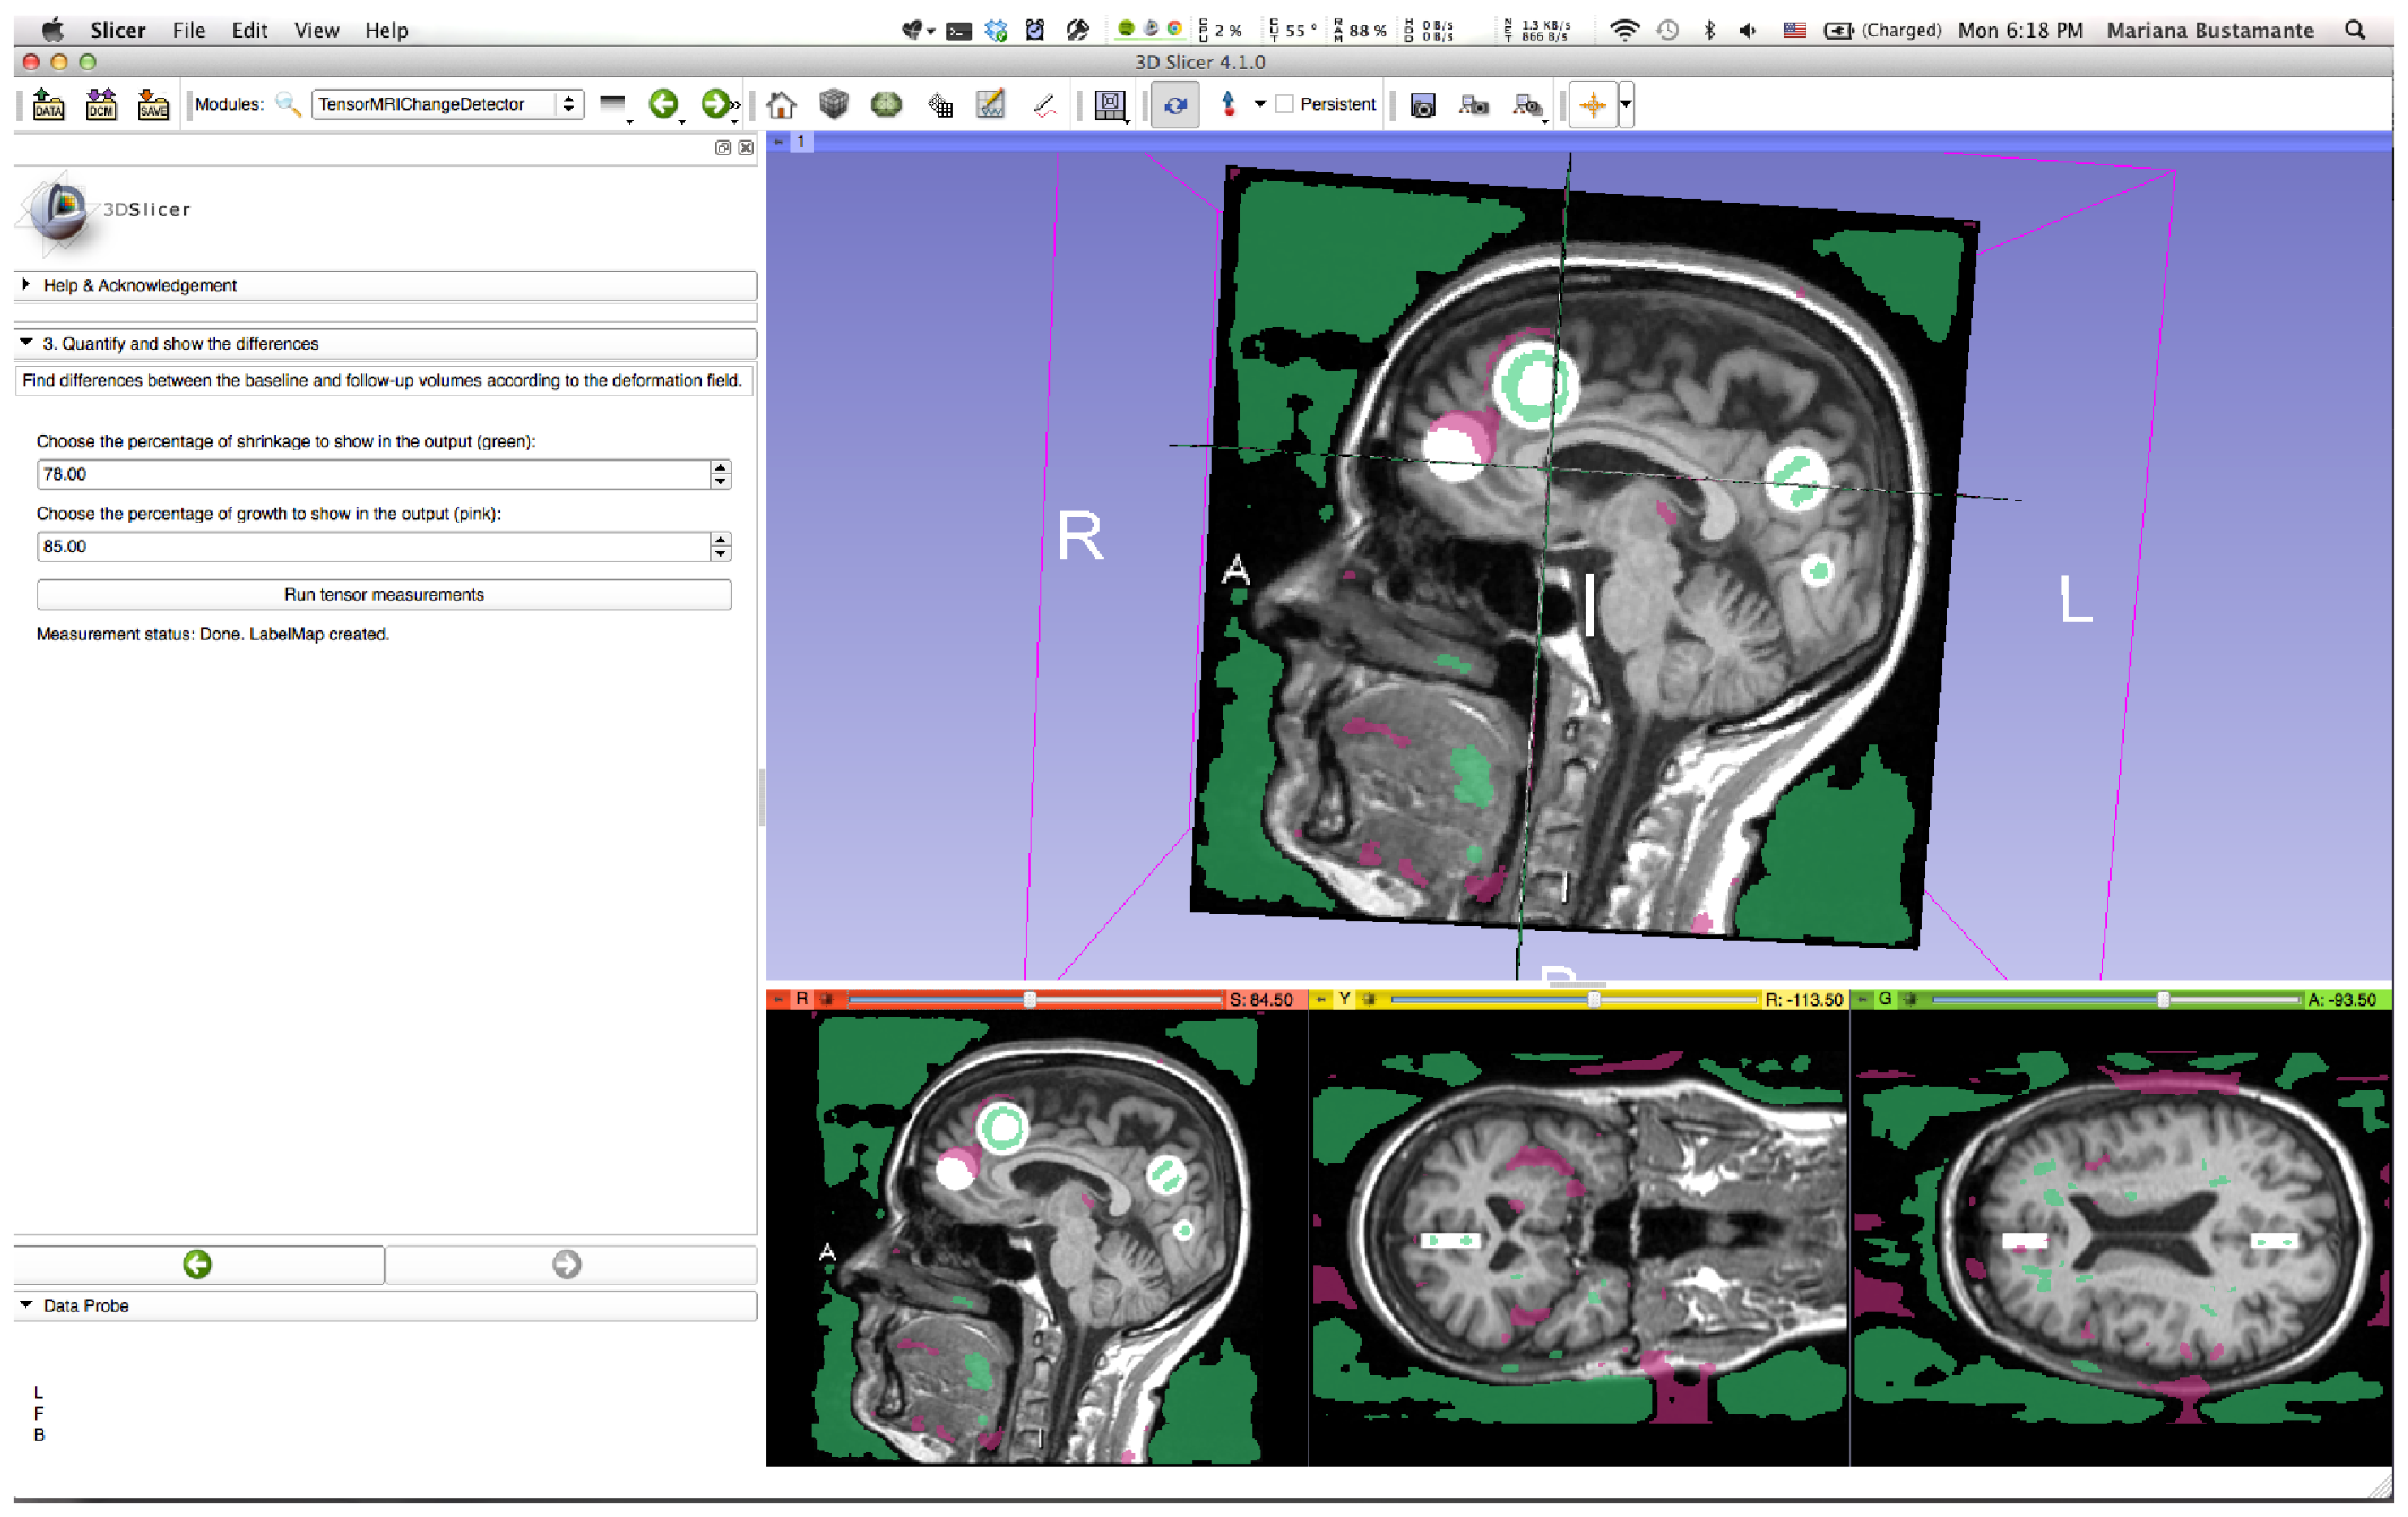
\includegraphics[scale=0.2]{/tensor_example/6.Result3.eps}
    \caption{Step 6: Interactive growth/shrinkage values}
    \label{tensor_ex_6}
  \end{figure}

\end{enumerate}


\subsubsection{Technical Details}
Like the voxel-based method, the user interface of the module is
written in \textit{Python} using some libraries from \textit{Qt} and
\textit{CTK}, being \textit{ctkWorkflowWidgetStep} from \textit{CTK}
the most important since it allows the creation of a ``step-by-step''
wizard.\\

The tensor measurements are written in \textit{C++} using
\textit{ITK}. It is the most important part of the method and it
includes the following functionalities:
\begin{itemize}
\item Computation of the \textit{Jacobian determinant} at each point
  in the deformation field by using the filter
  \textit{DisplacementFieldJacobianDeterminantFilter}.
\item Initially the Jacobian values are centered on $1.0$, this means
  that when the values are close to $1.0$ the change in the volume is
  nonexistent or small enough to be ignored. 

  In order to move the ``no-change-zone'' from $1.0$ to $0.0$, a
  \textit{logarithm} filter is applied on the Jacobian values.
  %TODO is there a better reason?
  
\item Computation of the \textit{Jacobian determinant} values that
  will be shown on the final result according to the percentages
  chosen by the user.
\item Creation of a label map with two colors that represent growth
  and shrinkage only showing the amount of values specified by the
  user.
\item Creation of a volume with all the values of the \textit{Jacobian
    determinant} for comparison with the previously described label
  map.
\end{itemize}
